\chapter{Gestión del tiempo}
%\paragraph{}WRITE HERE

\section{Descripción de actividades}


\subsection{Obtención de planos arquitectónicos}
\begin{itemize}
\item \textbf{Identificador: }1.1.1 A.
\item \textbf{Paquete de trabajo: }Planos arquitectónicos.
\item \textbf{Descripción: }Mediante una citación telemática o telefónica, se concierta una reunión con el Arquitecto de la edificación. En dicha reunión se obtendrán los planos arquitectónicos del edificio en fase de finalización de obra, dado que en esta fase no se modificará la edificación y se podrá ejecutar la instalación de la ICT sobre ellos.
\item \textbf{Responsable: }Director.
\item \textbf{Recursos materiales: }Para esta actividad no hará falta ningún recurso.
\item \textbf{Recursos humanos: }El director realizará esta actividad dedicándole 8 horas.
\item \textbf{Estimación de duración: }1 día.
\item \textbf{Secuencia de actividades: }Esta actividad no necesita de otra para ser iniciada, sino que es la primera actividad de la que procederán los siguientes paquetes de trabajo.
\end{itemize}

\subsection{Obtener medidas de potencia de señal}
\begin{itemize}
\item \textbf{Identificador: }1.1.2 D.
\item \textbf{Paquete de trabajo: }Evaluación de emplazamiento.
\item \textbf{Descripción: }Se evaluará, de manera presencial en la ubicación de la edificación, todos aspectos necesarios para la realización de los cálculos previos. Uno de estos aspectos será la obtención de las medidas de potencia de señal. Se medirá la potencia de señal recibida en varios puntos del emplazamiento y se estudiará cuál es el mejor lugar para la colocación de las antenas de la instalación RTV.
\item \textbf{Responsable: }Ingenieros e instaladores.
\item \textbf{Recursos materiales: }Para esta actividad será necesario un medidor de radiación electromagnética para observar la calidad de señal recibida y sus interferencias. Los ingenieros escogerán 5 lugares, previamente estudiados, para realizar las mediciones.
\item \textbf{Recursos humanos: }Esta tarea la realizarán los ingenieros(Ingeniero semi Senior) junto a los instaladores(Ingeniero Júnior, Ingeniero Técnico o ténico instalador). Cada ingeniero le dedicará 30 minutos por día y los instaladores 2 horas por día.
\item \textbf{Estimación de duración: }3-4 días.
\item \textbf{Secuencia de actividades: }Para hacer esta actividad es necesario que se hayan obtenido los planos arquitectónicos (paquete de trabajo 1.1.1). Tras esta actividad, ya se puede hacer los cálculos previos (paquete de trabajo 1.2.1).
\end{itemize}

\subsection{Elección del tipo de cableado}
\begin{itemize}
\item \textbf{Identificador: }1.2.1 A.
\item \textbf{Paquete de trabajo: }Cálculos previos.
\item \textbf{Descripción: }Para determinar el tipo de cableado, se deberá elegir dependiendo del lugar determinado donde se realizará la instalación. Hay que tener en cuenta distintos factores, entre ellos:
\begin{enumerate}
\item Carga de tráfico en la red.
\item Nivel de seguridad requerida en la red.
\item Distancia que debe cubrir el cable.
\item Opciones disponibles del cable.
\item Presupuesto para el cable.
\end{enumerate}
\item \textbf{Responsable: }Ingenieros.
\item \textbf{Recursos materiales: }Para esta actividad no hará falta ningún recurso.
\item \textbf{Recursos humanos: }Esta actividad será realizada por el ingeniero, le dedicará 3 horas diarias. en total dedicará 15 horas a esta actividad.
\item \textbf{Estimación de duración: }5 días.
\item \textbf{Secuencia de actividades: }Para esta actividad será necesario haber obtenido la aprobación de la evaluación de emplazamiento (paquete de trabajo 1.1.2).
\end{itemize}

\subsection{Entregar el proyecto a una entidad verificadora}
\begin{itemize}
\item \textbf{Identificador: }1.3.1 A.
\item \textbf{Paquete de trabajo: }COITT.
\item \textbf{Descripción: }El director de obra entregará el proyecto a una entidad verificadora, como el  Colegio Oficial de Ingenieros Técnicos en Telecomunicaciones(COITT). Esta entidad informará si se deben realizar cambios en el proyecto y, finalmente, confirmará la verificación del proyecto.
\item \textbf{Responsable: }Director de obra.
\item \textbf{Recursos materiales: }Es necesario tener redactado el proyecto.
\item \textbf{Recursos humanos:} El director de obra(Ingeniero Senior) realizará esta actividad. Dedicará 30 minutos diarios para leer las recomendaciones y corregir fallos que pueden aparecer en el documento.
\item \textbf{Estimación de duración: }1 semana.
\item \textbf{Secuencia de actividades: }Esta actividad se realiza cuando se haya acabado de redactar el proyecto(paquete de trabajo 1.2). Tras esta actividad se puede proceder a la ejecución e instalación(paquete de trabajo 1.4).
\end{itemize}

\subsection{Montaje de antenas}
\begin{itemize}
\item \textbf{Identificador: }1.4.2.1 A.
\item \textbf{Paquete de trabajo: }Antenas.
\item \textbf{Descripción: }La función principal de una antena receptora es convertir la energía electromagnética procedente de la emisora de televisión en una energía eléctrica que se pueda usar en los receptores de TV y radio. Los instaladores deberán realizar esta actividad, siempre utilizando las técnicas apropiadas(como se establece en el protocolo de instalación de antenas) y obteniendo las siguientes características de las antenas(al montarlas):
\begin{enumerate}
\item Buena captación de la señal.
\item Evitar ondas reflejadas.
\item Impedir reflexiones en el propio sistema.
\item Captar el mínimo posible de interferencias. 
\item Ser válida para el mayor número posible de canales.
\end{enumerate}
\item \textbf{Responsable: }Instaladores.
\item \textbf{Recursos materiales: }Serán necesarias herramientas tales como alicates, destornilladores, juego de llaves alen, llaves hexagonales, taladro, etc. (todos ellos específicos para la instalación de antenas). También será necesario equipamiento básico de seguridad para los instaladores, según la normativa de seguridad.
\item \textbf{Recursos humanos: }Esta actividad será realizada por los instaladores, cada instalador dedicará 6 horas diarias. En total hará cada uno 126 horas.
\item \textbf{Estimación de duración: }21 días
\item \textbf{Secuencia de actividades: }Esta actividad debe realizarse simultáneamente con las actividades de montaje (paquete de trabajo 1.4.2)
\end{itemize}

\subsection{Instalación del cableado}
\begin{itemize}
\item \textbf{Identificador: }1.4.3 A.
\item \textbf{Paquete de trabajo: }Canalización.
\item \textbf{Descripción: }Los instaladores realizarán la canalización de la edificación (canalización externa, de enlace, recinto de instalaciones de telecomunicación, unión a sistemas de captación, principal y secundaria). La canalización principal constará de cinco tubos de 50mm de diámetro (RTV, pares trenzados, coaxial, fibra óptica y uno de reserva). La canalización secundaria constará de tres tubos de 25mm de diámetro (pares trenzados y fibra, coaxial de servicios de TBA y coaxial de servicios de RTV). Si la distancia entre el registro secundario y de terminación de red supera los 15m, habrá de instalarse registros de paso que faciliten las tareas de instalación y mantenimiento.
\item \textbf{Responsable: }Instaladores.
\item \textbf{Recursos materiales: } Es necesario el material para realizar la canalización de la instalación: tubos de 50mm y de 25mm de diámetro para las canalizaciones principal y secundaria, cables de pares o pares trenzados, cables coaxiales, cables de fibra óptica y registros secundarios.
\item \textbf{Recursos humanos: }Esta actividad será realizada por los instaladores, cada instalador dedicará 6 horas diarias. En total hará cada uno 72 horas.
\item \textbf{Estimación de duración: }12 días
\item \textbf{Secuencia de actividades: }Esta actividad viene precedida de la tarea 1.4.2. Tras esta actividad, se realizarán los paquetes 1.4.4 y 1.5.
\end{itemize}

\subsection{Resolver dudas en el proceso de instalación}
\begin{itemize}
\item \textbf{Identificador: }1.4.5.1 B.
\item \textbf{Paquete de trabajo: }Supervisión.
\item \textbf{Descripción: }Los ingenieros deberán estar presentes en el proceso de instalación, para resolver las dudas que les puedan surgir a los instaladores. El director visitará la obra periódicamente (dos veces a la semana) por si su ayuda fuese necesaria. En caso de requerir la opinión del cliente para ciertos aspectos del montaje de la instalación, será el director el encargado de comunicarse con éste para conocer sus criterios y preferencias.
\item \textbf{Responsable: }Director e Ingenieros.
\item \textbf{Recursos materiales: }Ninguno.
\item \textbf{Recursos humanos:}Se requerirá al menos un ingeniero se encuentre en el edificio durante todo el proceso de instalación. Además el director deberá visitarlo periódicamente, lo que le supondrá 6 horas de trabajo a la semana. En total serán 210 horas de ingeniero junior y 42 horas de ingeniero senior (el director).
\item \textbf{Estimación de duración: }1 año, 1 mes y 11 días.
\item \textbf{Secuencia de actividades: } Esta actividad debe realizarse simultáneamente al proceso de instalación, lo que representa el conjunto de todas las actividades de (1.4).
\end{itemize}

\subsection{Realización del manual de usuario}
\begin{itemize}
\item \textbf{Identificador: }1.5 C.
\item \textbf{Paquete de trabajo: }Documentos finales.
\item \textbf{Descripción: }El director redactará el manual de usuario de la ICT que se ha realizado, siguiendo las indicaciones del Anexo VI de la Orden ITC/1644/2011. Dicho manual deberá incluir:
\begin{enumerate}
\item Identificación del edificio
\item Objetivo del documento
\item Introducción
\item Esquema de la instalación efectuada
\item Resumen de servicios instalados
\item Descripción de la instalación interior de usuario
\item Servidumbres
\item Garantía de la ICT
\item Documentación de las Instalaciones de Telecomunicación de la Edificación (ICT)
\item Recomendaciones de mantenimiento para las instalaciones
\end{enumerate}
Posteriormente a su redacción, se entregarán dos copias del manual de usuario (una en catalán y una en castellano) a la propiedad del edificio.
\item \textbf{Responsable: }Director
\item \textbf{Recursos materiales: }Se requerirá del uso de un PC con editor de texto y de una impresora con papel y tinta suficientes.
\item \textbf{Recursos humanos:}10 horas de trabajo del director (ingeniero senior)
\item \textbf{Estimación de duración: }2 días.
\item \textbf{Secuencia de actividades: }Esta actividad deberá realizarse después de haber terminado todas las actividades de montaje (1.4.2) y canalización (1.4.3) de la instalación. También es recomendable que se haya terminado la actividad de realización de pruebas (1.4.4 A).
\end{itemize}

\section{Cronograma del proyecto}

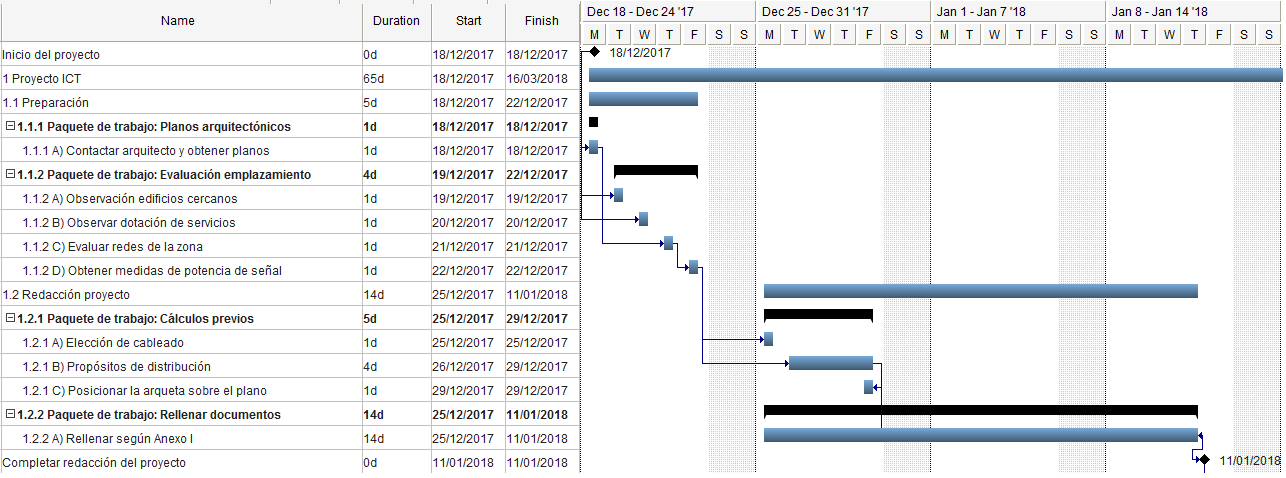
\includegraphics[scale=0.48]{project/images/c1.png} \\
\\
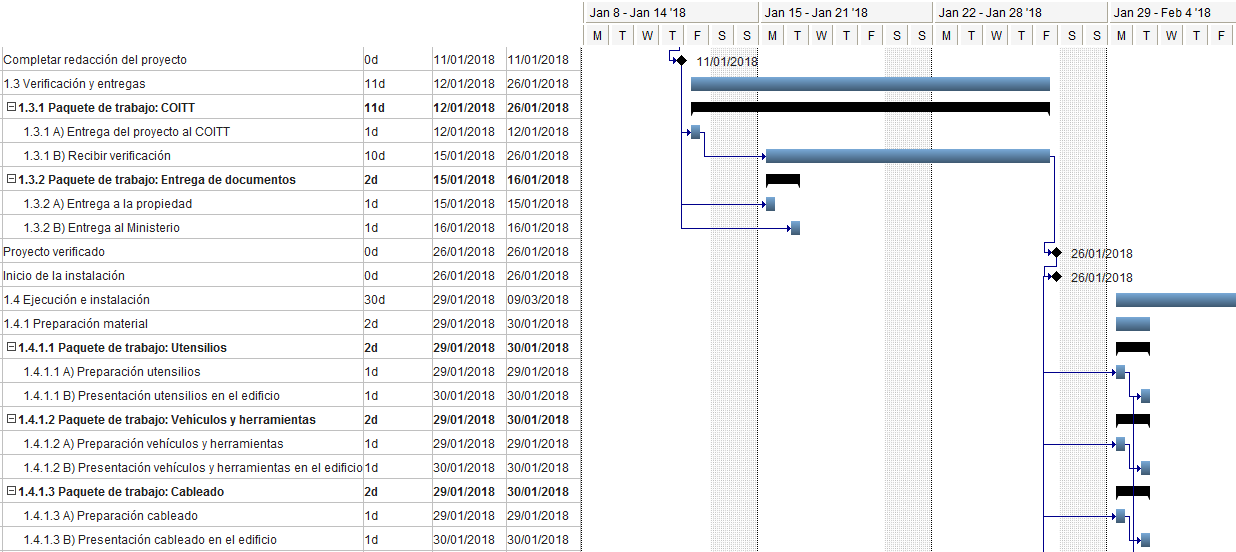
\includegraphics[scale=0.5]{project/images/c2.png} \\
\\
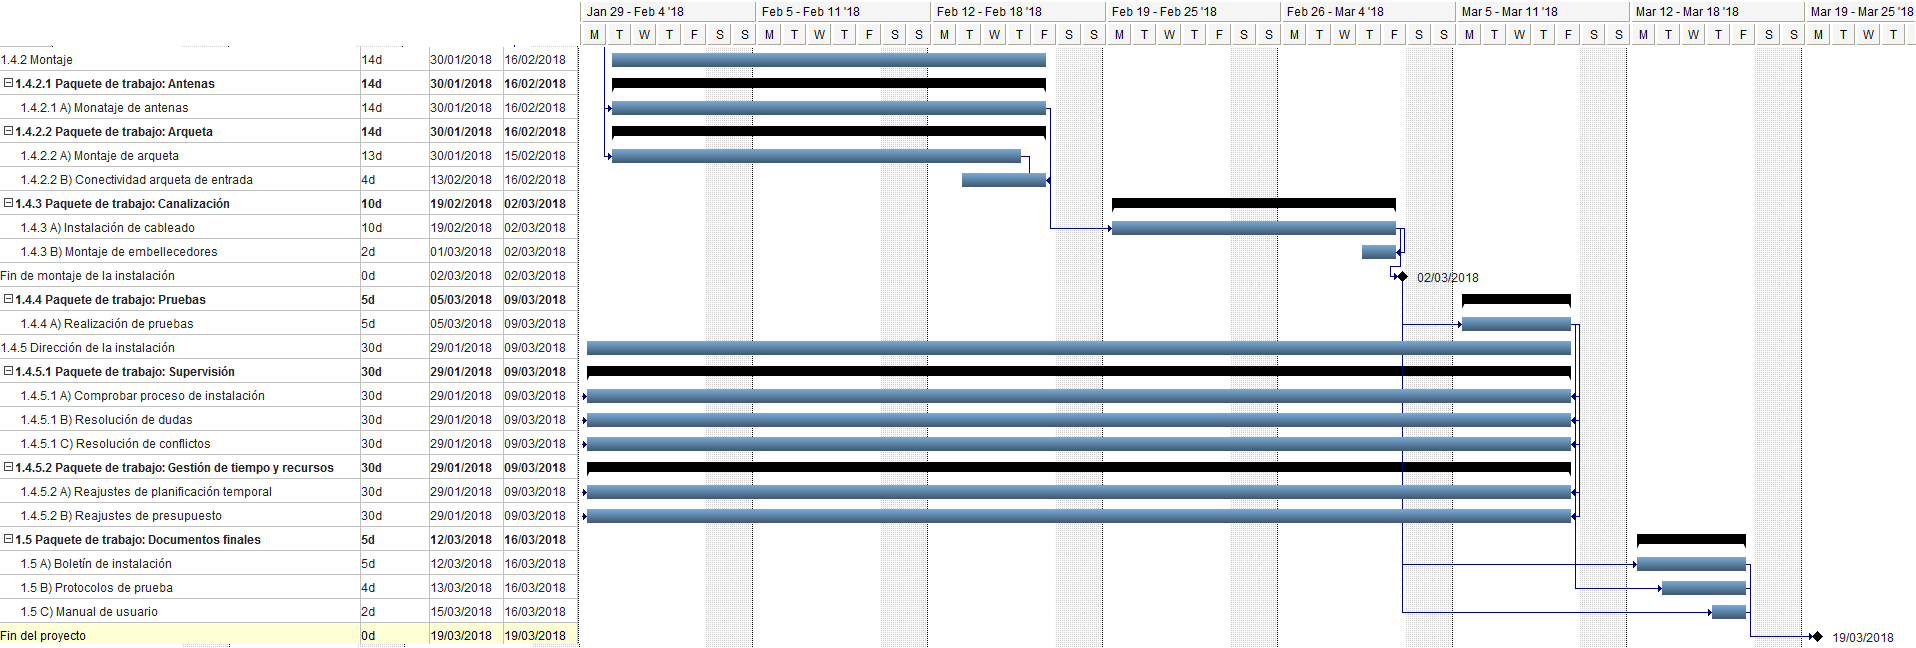
\includegraphics[scale=0.37]{project/images/c3.png} \\
